% Part: normal-modal-logic
% Chapter: syntax-and-semantics
% Section: relational-models

\documentclass[../../../include/open-logic-section]{subfiles}

\begin{document}

\olfileid{mod}{syn}{rel}

\olsection{Relational Models}

The basic concept of semantics for normal modal logics is that of a
\emph{relational model}. It consists of a set of worlds, which are
related by a binary ``accessibility relation,'' together with an
assignment which determines which !!{propositional variable}s count as
``true'' at which worlds.

\begin{defn}
  A \emph{model} for the basic modal language is a triple $\mModel{M}
  = \tuple{W, R, V}$, where
  \begin{enumerate}
  \item $W$ is a nonempty set of ``worlds,''
  \item $R$ is a binary accessibility relation on~$W$, and
  \item $V$ is a function assigning to each !!{propositional
    variable}~$p$ a set $V(p)$ of possible worlds.
  \end{enumerate}
  When $Rww'$ holds, we say that $w'$ is \emph{accessible
    from}~$w$. When $w \in V(p)$ we say $p$ is \emph{true at}~$w$.
\end{defn}

The great advantage of relational semantics is that models can be
represented by means of simple diagrams, such as the one in
\olref{fig:simple}. Worlds are represented by nodes, and world~$w'$ is
accessible from $w$ precisely when there is an arrow from~$w$
to~$w'$. Moreover, we write $p$ next to a world precisely when $w \in
V(p)$. \olref{fig:simple} represents the model with $W = \{w_1, w_2,
w_3\}$, $R = \{\tuple{w_1, w_2},\tuple{w_1, w_3}\}$, $V(p) = \{w_1,
w_2\}$, and $V(q) = \{w_2\}$.

\begin{figure}
  \begin{center}
    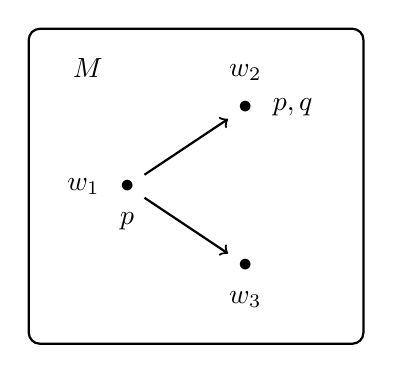
\begin{tikzpicture}[node distance=2cm, auto, thick]
      \node (w1) at (0, 1) [label=180:$w_1$, label=below:$p$]{$\bullet$}; 
      \node (w2) at (1.5, 2) [label=90:$w_2$, label=right:{$p, q$}]{$\bullet$}; 
      \node (w3) at (1.5, 0) [label=270:$w_3$] {$\bullet$}; \draw[->] (w1) to node {} (w2);
      \draw[->] (w1) to node {} (w3);
      \draw [rounded corners] (-1.25,-1) -- ++(0,4)  -- ++(4.25,0) -- ++(0,-4) --  cycle;
      \path node at (-0.5,2.5) {$\mModel{M}$};
    \end{tikzpicture}
  \end{center}
\caption{A simple model.}\ollabel{fig:simple}
\end{figure}

\end{document}
